% !TEX program = xelatex
%Wzór dokumentu
%tu zmień marginesy i rozmiar czcionki
\documentclass[a4paper,12pt]{article}
\usepackage{inputenc}[utf8]
\usepackage[margin=2.8cm]{geometry}
\usepackage[polish]{babel}

%Lepiej tego nie zmieniaj, jak co to dodawaj pakiety
\usepackage{titlesec}
\usepackage{titling}
\usepackage{fancyhdr}
\usepackage{mdframed}
\usepackage{graphicx}
\usepackage{amsmath}
\usepackage{amsfonts}
\usepackage{multicol}
\usepackage{multirow}
\usepackage{listings}
\usepackage{caption}
\usepackage{float}
\usepackage{pdfpages}
\usepackage{tikz}
	\usetikzlibrary{arrows}
	\usetikzlibrary{patterns}
	\usetikzlibrary{decorations.pathmorphing}
\usepackage{pgf}
\usepackage[section]{placeins}



%inny wygląd
%\usepackage{tgbonum}


\usepackage{hyperref}
\hypersetup{
    colorlinks=true,
    linkcolor=blue,
    filecolor=magenta,      
    urlcolor=cyan,
}

\urlstyle{same}
%Zmienne, zmień je!
\graphicspath{ {./ilustracje/} }
\title{Wyznaczanie wartości przyspieszenia ziemskiego metodą spadku swobodnego}
\author{Grzegorz Koperwas}
\date{\today}

%lokalizacja polska (odkomentuj jak piszesz po polsku)

\usepackage{polski}
\usepackage[polish]{babel} 
\usepackage{indentfirst}
\usepackage{icomma} 

\brokenpenalty=1000
\clubpenalty=1000
\widowpenalty=1000    

%nie odkometowuj wszystkiego, użyj mózgu
%\renewcommand\thechapter{\arabic{chapter}.}
\renewcommand\thesection{\arabic{section}.}
\renewcommand\thesubsection{\arabic{section}.\arabic{subsection}.}
\renewcommand\thesubsubsection{\arabic{subsubsection}.}

%Makra

\newcommand{\obrazek}[2]{
\begin{figure}[h]
    \centering
    \includegraphics[scale=#1]{#2}
\end{figure}
}     

\newcommand{\stopnie}{\ensuremath{^{\circ}}}

\newcommand{\twierdzonko}[1]{
    \begin{center}
    \begin{mdframed}
    #1
    \end{mdframed}          
    \end{center}
} 

\newcommand{\dwanajeden}[2]{
\ensuremath \left( \begin{array}{c}
    #1\\
    #2
\end{array} \right)
}  

%Stopka i head (sekcja której nie powinno się zmieniać)
\pagestyle{fancy}
\fancyhead{}
\fancyfoot{}

%Zmieniaj od tego miejsca
\rfoot{\thepage}
\lfoot{}
\lhead{}
\rhead{Ostatnia edycja: \today}
\renewcommand{\headrulewidth}{1pt}
\renewcommand{\footrulewidth}{1pt}


\begin{document}
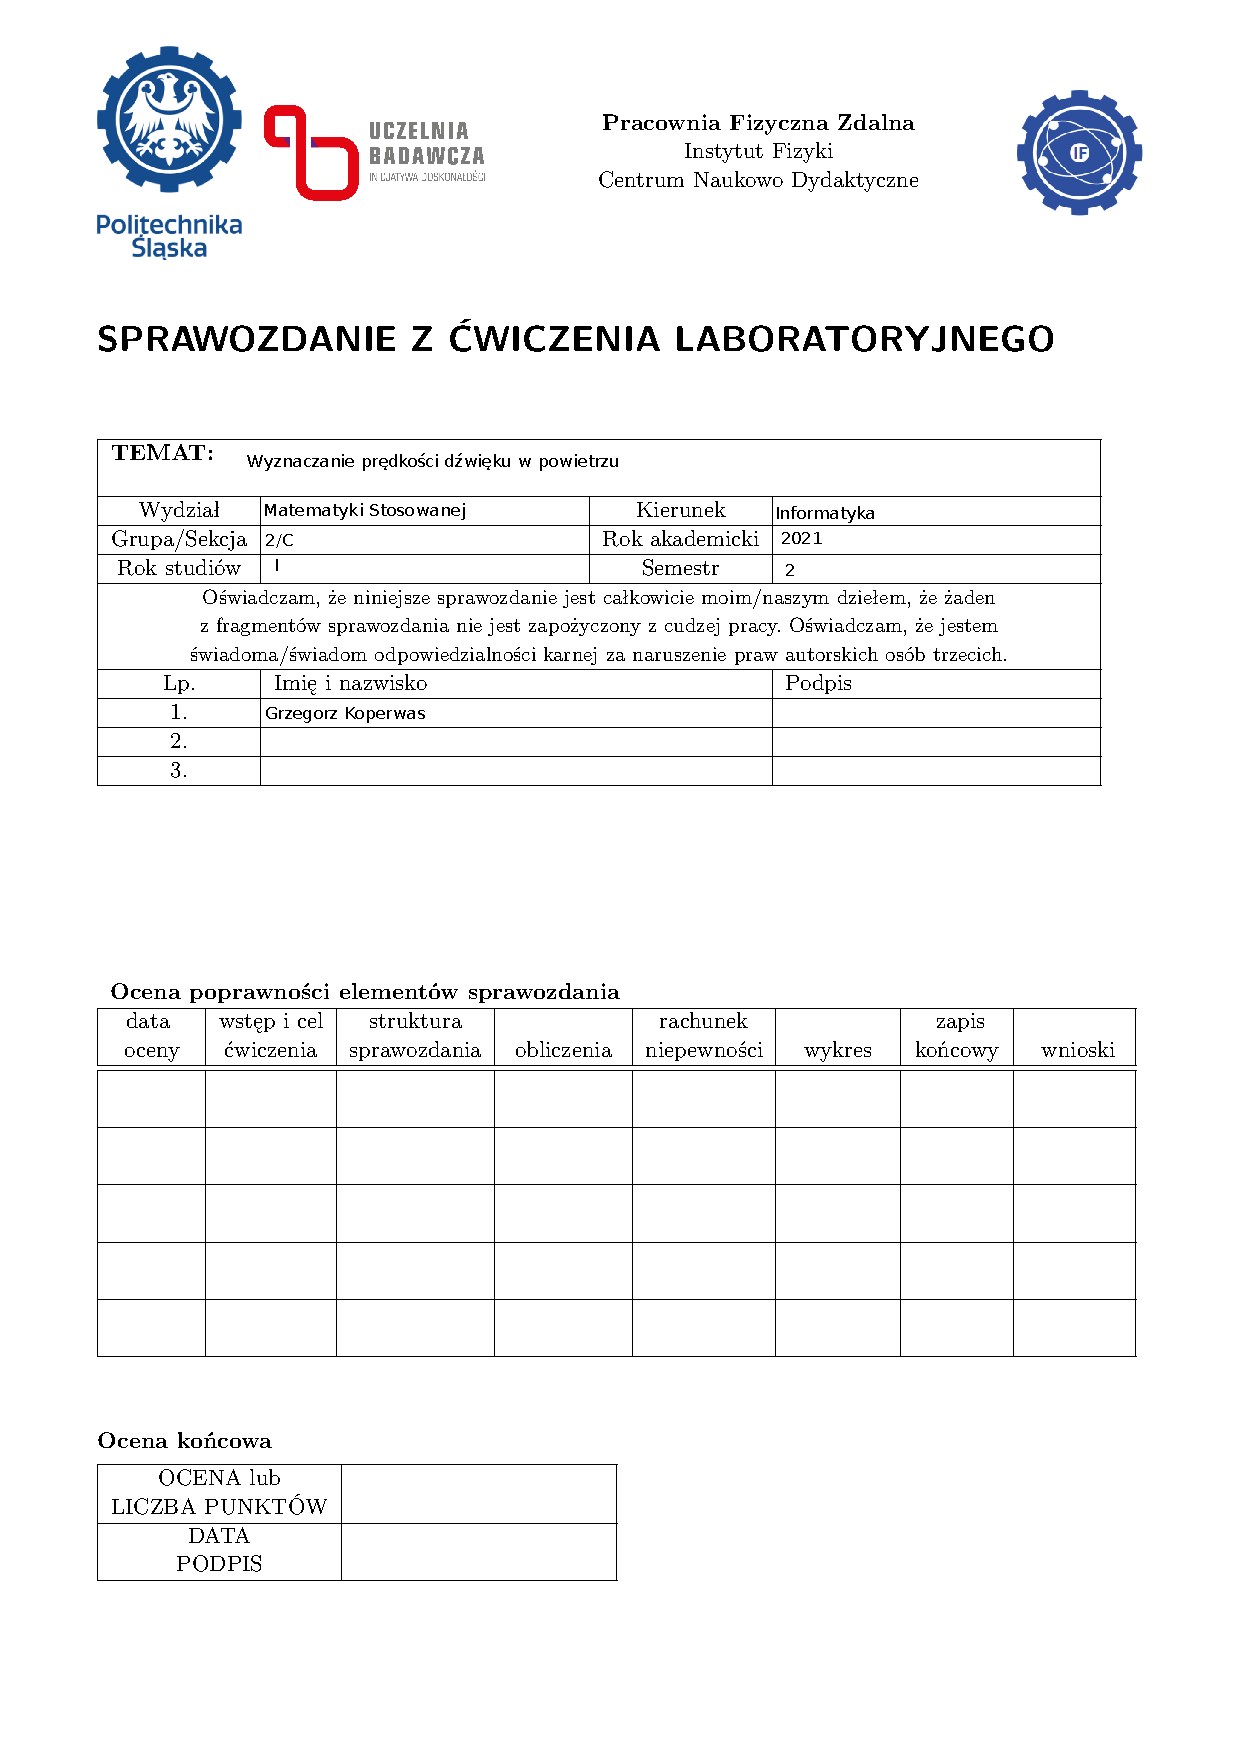
\includepdf[pages=-]{PFZ-StrTytulowa.pdf}
\section{Wstęp teoretyczny}

Celem doświadczenia jest pomiar prędkości dźwięku w powietrzu, poprzez mierzenie różnicy czasu między dwoma zarejestrowanymi przez urządzenia pomiarowe dźwiękami, które zostały wywołane tak jak na rysunku \ref{rys:układ}.

\begin{figure}[h]
    \begin{tikzpicture}
        \foreach \i in {1, 2}
        {
            \node[draw] at (\i * 10, 0) {\i};
            \draw[dashed, thin] (\i * 10, 1) -- (\i * 10, 0.3);
        }
        \draw[<->, thin] (10, 1) -- (20, 1) node [above ,pos=.5] {$d$};
        \fill (10.5, 0) circle (.1);
        \draw (10.5, 0) circle (.20);
        \foreach \i in {1, ..., 5}
        {
            \draw (10 + \i, 0) arc (0:30:1);
            \draw (10 + \i, 0) arc (0:-30:1);
        }
    \end{tikzpicture}
    \begin{tikzpicture}
        \foreach \i in {1, 2}
        {
            \node[draw] at (\i * 10, 0) {\i};
            \draw[dashed, thin] (\i * 10, 1) -- (\i * 10, 0.3);
        }
        \draw[<->, thin] (10, 1) -- (20, 1) node [above ,pos=.5] {$d$};
        \fill (19.5, 0) circle (.1);
        \draw (19.5, 0) circle (.20);
        \foreach \i in {1, ..., 5}
        {
            \draw (20 - \i, 0) arc (0:30:-1);
            \draw (20 - \i, 0) arc (0:-30:-1);
        }
    \end{tikzpicture}
    \centering
    \caption{Układ pomiarowy}\label{rys:układ}
\end{figure}

Urządzenie 1 zaczyna rejestruje dźwięk natychmiastowo, natomiast urządzenie 2 dopiero po czasie $t_r$. W przypadku drugiego dźwięku sytuacja jest odwrotna, urządzenie 2 rejestruje go natychmiastowo, a urządzenie 1, jako iż $d = const.$, rejestruje go po czasie $t_r$.

Niech $T$ to bezwzględny odstęp w czasie między dźwiękami:

\begin{gather*}
    \left\{ \begin{array}{l}
        t_1 = T + t_r\\
        t_2 = T - t_r
    \end{array} \right.\\
    t_1 - t_2 = 2\cdot t_r\\
    t_r = \frac{t_1 - t_2}{2}
\end{gather*}

Dźwięk przebywa odległość $2d$ w czasie $2 t_r$:

\begin{align*}
    v &= \frac{2d}{2 t_r}\\
    v &= \frac{2d}{t_1 - t_2}
\end{align*}

\clearpage

\section{Wyniki pomiarów}

\begin{table}[h]
	\begin{tabular}{|l|l|l|l|}
		\hline
		$t_1 [s] \pm 0,001 s$	& $t_2 [s] \pm 0,001 s$ & $t_1 - t_2$ & v $\left[\frac{m}{s^2}\right]$ \\\hline\hline
6,915	& 6,885	& 0,030	& 333,333 	\\\hline
6,780	& 6,745	& 0,035	& 285,714 	\\\hline
6,112	& 6,118	& -0,006	& -1666,667 	\\\hline
6,805	& 6,757	& 0,048	& 208,333 	\\\hline
6,892	& 6,861	& 0,031	& 322,581 	\\\hline
7,783	& 7,755	& 0,028	& 357,143 	\\\hline
8,082	& 8,057	& 0,025	& 400,000 	\\\hline
8,413	& 8,371	& 0,042	& 238,095 	\\\hline
8,603	& 8,537	& 0,066	& 151,515 	\\\hline
7,678	& 7,597	& 0,081	& 123,457 	\\\hline
	\end{tabular}
	\centering
	\caption{Pomiary dla $5m\; \pm 5cm$}
\end{table}

\begin{table}[h]
	\begin{tabular}{|l|l|l|l|}
		\hline
		$t_1 [s] \pm 0,001 s$	& $t_2 [s] \pm 0,001 s$ & $t_1 - t_2$ & v $\left[\frac{m}{s^2}\right]$ \\\hline\hline
5,274	& 5,283	& -0,009	& -666,667 	\\\hline
5,243	& 5,236	& 0,007	& 857,143 	\\\hline
5,082	& 5,085	& -0,003	& -2000,000 	\\\hline
4,852	& 4,836	& 0,016	& 375,000 	\\\hline
6,154	& 6,140	& 0,014	& 428,571 	\\\hline
5,416	& 5,404	& 0,012	& 500,000 	\\\hline
4,774	& 4,737	& 0,037	& 162,162 	\\\hline
5,129	& 5,108	& 0,021	& 285,714 	\\\hline
5,154	& 5,120	& 0,034	& 176,471 	\\\hline
4,325	& 4,307	& 0,018	& 333,333 	\\\hline
	\end{tabular}
	\centering
	\caption{Pomiary dla $3m\; \pm 5cm$}
\end{table}

\section{Przetwarzanie danych}

\begin{table}[p]
\centering
\begin{tabular}{|l|l|l|l|l|l|l|}
\hline
$d\; \left[m\right] \pm 0,050m$ & $\Delta t \left[s\right]$ & $u(\Delta t) \left[s\right]$ & $u(d) \left[m\right]$ & $v \left[\frac{m}{s}\right]$ & $u(v) \left[\frac{m}{s}\right]$ & $u^{-2}(v) \left[\frac{s^2}{m^2}\right]$ \\ \hline\hline
5,000 & 0,030  & 0,032 & 0,050 & 333,3   & 1,1  & 0,90 \\ \hline
5,000 & 0,035  & 0,032 & 0,050 & 285,7   & 0,9  & 1,22 \\ \hline
5,000 & -0,006 & 0,032 & 0,050 & -1666,7 & 5,3  & 0,04 \\ \hline
5,000 & 0,048  & 0,032 & 0,050 & 208,3   & 0,7  & 2,30 \\ \hline
5,000 & 0,031  & 0,032 & 0,050 & 322,6   & 1,0  & 0,96 \\ \hline
5,000 & 0,028  & 0,032 & 0,050 & 357,1   & 1,1  & 0,78 \\ \hline
5,000 & 0,025  & 0,032 & 0,050 & 400,0   & 1,3  & 0,62 \\ \hline
5,000 & 0,042  & 0,032 & 0,050 & 238,1   & 0,8  & 1,76 \\ \hline
5,000 & 0,066  & 0,032 & 0,050 & 151,5   & 0,5  & 4,35 \\ \hline
5,000 & 0,081  & 0,032 & 0,050 & 123,5   & 0,4  & 6,56 \\ \hline
3,000 & -0,009 & 0,032 & 0,050 & -666,7  & 3,5  & 0,08 \\ \hline
3,000 & 0,007  & 0,032 & 0,050 & 857,1   & 4,5  & 0,05 \\ \hline
3,000 & -0,003 & 0,032 & 0,050 & -2000,0 & 10,5 & 0,01 \\ \hline
3,000 & 0,016  & 0,032 & 0,050 & 375,0   & 2,0  & 0,26 \\ \hline
3,000 & 0,014  & 0,032 & 0,050 & 428,6   & 2,3  & 0,20 \\ \hline
3,000 & 0,012  & 0,032 & 0,050 & 500,0   & 2,6  & 0,14 \\ \hline
3,000 & 0,037  & 0,032 & 0,050 & 162,2   & 0,9  & 1,37 \\ \hline
3,000 & 0,021  & 0,032 & 0,050 & 285,7   & 1,5  & 0,44 \\ \hline
3,000 & 0,034  & 0,032 & 0,050 & 176,5   & 0,9  & 1,16 \\ \hline
3,000 & 0,018  & 0,032 & 0,050 & 333,3   & 1,8  & 0,32 \\ \hline
\end{tabular}
\caption{Dane przetworzone}
\label{tab:proc}
\end{table}

Obliczamy średnią ważoną (i jej niepewność) dla wartości z tablicy \ref{tab:proc} gdzie $v > 0$.
\clearpage

\section{Wnioski}

Prędkość dźwięku według danych z tablicy \ref{tab:proc} to:

\[\bar{v} = 205 \frac{m}{s};\; u\left(\bar{v}\right) = 42 \frac{m}{s}\]

Prędkość dźwięku w temperaturze $22\stopnie C$ wynosi, według tablic, $344,31 \frac{m}{s}$. Zatem:

\begin{align*}
    \left| 205 - 344,31 \right| &< 2 \cdot 42\\
    139,31 &\not < 84
\end{align*}

Zmierzona wartość nie jest zgodna z wartościami tablicowymi.

\section{Sposoby na zmniejszenie niepewności}

Głównym źródłem błędów był niestaranny pomiar odległości między urządzeniami pomiarowymi, który nie zawsze był odległością jaką pokonywał dźwięk. niemożliwe jest (lub nie jest bezpieczne) wywoływanie dźwięku młotkiem w odległości mniejszej niż 10-15cm od urządzenia pomiarowego. Stworzenie profesjonalnego urządzenia złożonego z mikrofonu i głośnika w najbliższej jak to możliwe odległości pozwoliło by wyeliminować błędy w tym przypadku.

Innym źródłem błędów była nieidealna procedura pomiarowa, gdzie jedno z urządzeń było telefonem z uruchomioną aplikacją \texttt{phyphox}, która, z powodu nie znanej do końca metody pomiaru, mogła być źródłem błędów. Zastąpienie jej komputerem z mikrofonem, i manualnym odczytem czasu w programie \texttt{Audacity}, mogło by pozwolić na większą dokładność pomiaru.

\end{document}
